\documentclass[journal]{./IEEE/IEEEtran}
\usepackage{array}
\usepackage{cite,graphicx}
\usepackage{url}

\newcommand{\SPTITLE}{EDSAan: A Mobile Navigation System for the EDSA Carousel Busway }
\newcommand{\ADVISEE}{George O. Jaime III}
\newcommand{\ADVISER}{Assoc. Prof. Concepcion L. Khan}

\newcommand{\BSCS}{Bachelor of Science in Computer Science}
\newcommand{\ICS}{Institute of Computer Science}
\newcommand{\UPLB}{University of the Philippines Los Ba\~{n}os}
\newcommand{\REMARK}{\thanks{Presented to the Faculty of the \ICS, \UPLB\
                             in partial fulfillment of the requirements
                             for the Degree of \BSCS}}
        
\markboth{CMSC 190 Special Problem, \ICS}{}
\title{\SPTITLE}
\author{\ADVISEE~and~\ADVISER%
\REMARK
}
\pubid{\copyright~2025~ICS \UPLB}

%%%%%%%%%%%%%%%%%%%%%%%%%%%%%%%%%%%%%%%%%%%%%%%%%%%%%%%%%%%%%%%%%%%%%%%%%%

\begin{document}

% TITLE
\maketitle

\begin{abstract}
This study presents the development and evaluation of EDSAan, a mobile application designed to assist commuters of the EDSA Carousel bus system in Metro Manila. The app aims to improve the commuting experience by providing real-time bus stop tracking, offline GPS navigation, and location-based notifications. To assess its effectiveness, three main objectives were evaluated: the usability of the app’s interface for EDSA Carousel travel, the functionality of its offline GPS features, and the overall user satisfaction and usability of the app.

Evaluation data were collected through a custom questionnaire and the System Usability Scale (SUS), with a total of 179 valid responses analyzed. The results showed high levels of agreement across all three objectives, with average Likert scale ratings ranging from 4.45 to 4.76 out of 5. The SUS yielded an average score of 85.52, indicating excellent usability. Additionally, the researcher conducted a personal test by using the app across all 24 EDSA Carousel stations, confirming its real-world performance through video documentation.

Overall, the findings suggest that EDSAan is a highly usable and reliable tool for daily commuters, especially those who rely on offline navigation. The app demonstrates strong potential to support urban transportation needs and improve the commuting experience along the EDSA Carousel route.
\end{abstract}

% INTRODUCTION
\section{Introduction}

\subsection{Background of the Study}
The EDSA Carousel is a Bus Rapid Transit (BRT) with a route that traverses the entirety of Epifanio de los Santos Avenue (EDSA) and further reaches out to Parañaque Integrated Terminal Exchange, commonly known as PITX. This transportation system operates 24 hours on a dedicated roadway and has been reported to service 389,579 passengers daily on average in 2022 \cite{Ref:006}. With the EDSA Carousel being a BRT, the buses can only load and unload passengers on specified stations and behave more like a railway.

For commuters in the Philippines, the existing routine for public utility buses (PUBs) is employing conductors and drivers verbally announcing the upcoming bus stops \cite{Ref:004}, with the hopes that the passengers will take notice. Regulated fares also resulted in a more aggressive competition, forcing these buses to rush and cram passengers tightly together.

The convention for getting off the bus constitutes the conductors to shout the stops to the passengers, and the passengers to shout “para” to the conductors or drivers, and the lack of a proper environment in effectively communicating with the passengers risks the passengers missing their destinations \cite{Ref:002}.  In fact, not only does this happen a lot, but also in different parts of the world. Sigurd D’hondt’s study (2009) observed similar experiences in Dar-es Salaam minibuses (16-seater Toyota Hiace) in Tanzania, where there is always a conflict in verbal communication between the conductor and the passenger.
A study on passenger expectations for EDSA Carousel \cite{Ref:001} yielded findings that indicate the need for a proper indicator showing travel status catered to passengers. In addition, public transportation applications on mobile such as Sakay.ph (A multi-modal transportation app for Metro Manila \cite{Ref:015}) and ikotMNL (an LRT-1-focused transportation app \cite{Ref:008}) have always been reliant on constant internet connectivity to provide service to their users, and will prove to be challenging for passengers who cannot afford to top-up for telcos’ internet data services. The lack of a solution for these kinds of needs poses a problem for the commuters.


\subsection{Statement of the Problem}
The traditional method of information system on PUBs will most likely result in an unpredictable journey especially for first-time commuters, causing passengers to be uncomfortable and miss their stop since most of them are packed together in the aisle when the seats are full \cite{Ref:004}.
In rush hour, this situation disconnects the passengers from the outside of the bus or even the conductor, making it difficult for them to perceive information about their current location and therefore, potentially miss their stops.

\subsection{Objectives of the Study}
The main objective of this study is to develop a mobile application that determines the passengers’ location along the EDSA Carousel and have the capability to report to the user when their specified stop is nearing.

Specifically, the study aims to:
\begin{enumerate}
    \item Develop a mobile app interface tailored for navigating the EDSA Carousel Busway,
    \item determine the effectivity of smartphone’s offline GPS along EDSA Busway stations, in a poor network situation,
    \item determine the overall usability of EDSAan for the commuters.
\end{enumerate}

\newpage

\subsection{Significance of the Study}
In line with the nature of public transportation in the Philippines, developing an effective mobile application that will signal the passengers of their current location in the EDSA Busway will help alleviate their struggles by providing another channel of information for the passengers to rely on. Using the features of smartphones to the commuters’ advantage will help develop a travel information system that can be reliable on various situations. 


\subsection{Scope and Limitations}
EDSAan was developed under the React Native framework and will be exclusively tested on a smartphone with an Android operating system. This study evaluated the application’s usability through the commuters of the EDSA Carousel of all genders and ages.
The mobile application only caters to the EDSA Busway’s route and not the MRT Line 3 above it. The study does not address other forms of customer expectations for the busway such as pollution and pricing. Developing a version of the application for iOS will not be considered at this point due to budget constraints.



% REVIEW OF RELATED LITERATURE

\section{Review of Related Literature}
Several studies and digital resources relevant to this research have focused on areas such as public transportation, mobile development, and usability evaluation. Although each work varies in its chosen methodology and implementation, they share a common objective: to assist researchers and developers in designing mobile applications and understanding the broader context of public transportation in the Philippines.

It is important to know that some literature reviewed in this study does not necessarily comply with the 10-year validity consensus in research. However, these studies have been shown to be relevant for the current situation in Philippine public transportation and the technologies used to develop EDSAan.

A study by Aguilar et al. \cite{Ref:001} revealed various passenger expectations about the relatively young EDSA carousel. The assessment is mainly divided into seven criteria, each having their own sub criteria. Pricing and budgeting were under the affordability criteria, journey satisfaction was under reliability,  ease of access was under accessibility, pollution experience was under environment, customer service was under tangibility, bus stop condition and bus condition were under comfortability, and personal safety and security under safety.

In the category of bus condition, the factor analysis revealed the need for key performance indicators (KPIs) on buses to show their travel status. These metrics can improve passenger comfort and help guide the study toward its objectives. They also help define the study’s limitations in relation to other factors in passenger expectations.

The situation of public utility buses (PUB) in the Philippines is comparable to that of mini buses in Dar-es-Salaam, a city in Tanzania that is a country located in Eastern Africa. D’hondt’s \cite{Ref:005} spatial analysis on their kind of public transportation have provided valuable insights regarding the use of space and how it affects the experience of passengers.

One of the findings showed that information is often passed along until it reaches the conductor, who then alerts the driver about passengers preparing to get off. Passengers also tend to keep track of others' drop-off points, a routine that is common among Filipino commuters who may want to adjust their seats ahead of time. Because of how crowded and busy the inside of the bus can be, passengers sometimes lose awareness of their surroundings. This can lead to missed stops or confusion among those on board. These are considered “deviant” cases in this study, meaning situations that deviate from the usual drop-off routine. Such cases, which reflect the real experience of commuting in Philippine buses, highlight the need for a comprehensive mobile application designed specifically for the EDSA Carousel Busway.

A related study by Jacob et al. \cite{Ref:009} about a mobile application that uses haptic feedback (vibrations) addresses similar concerns and was conducted to the benefit of the passengers. The system employs a similar concept to the mobile application that was developed, utilizing GPS functionality of smartphones, prompting users to select for destination, and giving feedback upon the user for estimated arrival.

The mobile application in the previous study did not undergo extensive real-world usability testing, which was the main gap that this study aimed to address. However, several findings from that research were used in the development of our mobile application. One key insight was that the most preferred types of feedback by respondents were displaying the user’s position on a map and providing vibration alerts to notify them of their bus stop. These insights were helpful in designing effective features for our transport-focused application.

In alignment with Jacob et al.’s gap in their paper lacking a proper usability testing, our study intends to follow Mifsud’s guide \cite{Ref:013} on testing mobile applications. The guide provides valuable information on the preliminaries needed, including a usability test plan containing the following: objectives, tasks to be performed by the respondent, documents (such as consent forms and questionnaires), participants, and test methods.

It is also important to determine the optimal number of respondents, as there is no clear consensus on how many evaluators are needed to achieve a good detection rate for usability issues \cite{Ref:007}. In a 2010 study by Hwang and Salvendy \cite{Ref:007}, regression analysis was performed on discovery rates from various usability evaluation experiments conducted over the years.

Their analysis has predicted an optimal number of test users to be 9 for Think Aloud Evaluation, 8 for Heuristic Evaluation, and 11 for Cognitive Walkthrough. These findings have derived a conclusion of having 10±2 as the optimal number of samples in evaluating software to detect at least 80\% of the usability problems, contrary to the widely accepted 4±1 often used by the community.

A usability analysis conducted by Toledo, Salgado, Gozum, and Custodio \cite{Ref:018} for Sakay.ph was also an inspiration for the study’s methodology, because it also falls under public transport and has features similar to ones to be implemented on our mobile app. Sakay.ph focuses on getting you from point A to point B anywhere in Metro Manila, by providing a comprehensive map that shows the available routes and the nearest transfer points when using public transportations.

One valuable finding from the study was the improper use of icons in the Sakay.ph interface—for example, some elements appeared clickable but did not perform any action. This insight helped guide our study in improving the user experience by providing more useful information for each bus stop, such as nearby dining options, places to visit, accommodations, and other relevant details.

To avoid the majority of usability problems in the first place, the developed mobile app should follow an intuitive design. Babich discussed five basic patterns for mobile navigation \cite{Ref:003} and their pros and cons to enable developers to weigh their decisions on implementing an effective user interface depending on different situations. These five patterns include the Hamburger Menu, Tab Bar, Priority+, Floating Action Button, and Full-Screen Navigation.

The Tab Bar provides upfront navigation options to the user on the main interface. With the option cells being placed side by side, its high discoverability makes the Tab Bar a rather good navigation system on the top level, as long as it does not have too many items, otherwise, the icons will look crammed together.

Taking these qualities into account, a clean fullscreen navigation paired with a tab bar is the most suitable design for EDSAan. Showing the main features right away makes the app easier to use for commuters and provides a natural way to navigate using simple and intuitive buttons. This approach is similar to the design used in the ikotMNL app for LRT passengers \cite{Ref:008} in Metro Manila.

Usability of a mobile app also relies on its ability to perform in various situations, and that includes the instability or absence of an internet connection. Surfshark’s 2023 Digital Quality of Life Index report \cite{Ref:016} has placed the Philippines on 104th out of 121 countries for internet affordability, a problem that lingers in our commuters.

EDSAan’s ability to run offline increases its usability and makes it more helpful for passengers. In developing an offline navigation system specifically for the EDSA Carousel route, a related study by Prathilothamai et al. \cite{Ref:014} shows that navigation is still possible even in areas without internet access or when connectivity is turned off.

With the GPS sensors in smartphones remaining functional in the absence of the internet, their mobile app continues to guide the user, with the premise that the area to be walked on should have been downloaded in the first place. This is not a problem for the EDSA route, as the GPS coordinates of bus stops remain absolute all throughout the route and comes pre-loaded with the app already.

Insights from studies on public transport, usability, and offline mobile systems highlight the need for intuitive, accessible tools to aid commuters. In areas with unreliable internet, such as Metro Manila, offline functionality and user-friendly design are essential. This study builds on those findings to improve the commuting experience on the EDSA Carousel through a practical, commuter-focused mobile solution.

% METHODOLOGY

\section{Materials and Methods}

\subsection{Development Devices}

The devices used to develop and test the mobile application have the following specifications:\\\\
1) Lenovo Thinkpad X270
\begin{itemize}
  \item Processor: Intel Core i5 7200U
  \item RAM: 16GB
  \item Storage: 512GB NVME SSD
  \item Operating System: Linux [Ubuntu 22.04]
\end{itemize}
2) Infinix Smart 8
\begin{itemize}
  \item CPU: Unisoc T606
  \item RAM: 4GB
  \item Storage: 128GB
  \item Operating System: Android 13\\
\end{itemize}


\subsection{Development Tools:}
The following tools were used in developing the application:
\begin{enumerate}
   \item \textbf{Visual Studio Code:} a code editor created by Microsoft that supports vast features, including but not limited to extensions, integrated terminal, code highlighting, debugging, and version control.
   \item \textbf{React Native:} a development framework that utilizes Javascript as its programming language and exports projects for multiple platforms. Created by Meta (formerly known as Facebook), it offers a familiar code structure similar to the ones used in web development, but renders the applications in the platforms’ native code. React Native also supports the use of libraries created by the community, allowing for efficient development.
   \item \textbf{Git:} a free and open-source distributed version control system designed to track changes in source code during software development.
   \item \textbf{Expo:} an open-source framework and platform for building universal React applications. It simplifies the development of mobile apps by providing a set of tools, libraries, and services that work out of the box with React Native.
   \item \textbf{Photopea:} a free, web-based image editor that supports advanced photo and graphic editing directly in the browser.
   

 \end{enumerate}

\subsection{Feature Set}
The mobile application is composed of the following features:
\newline

\subsubsection{\textbf{Choose Destination}}

\begin{figure}[htbp]
  \centering
  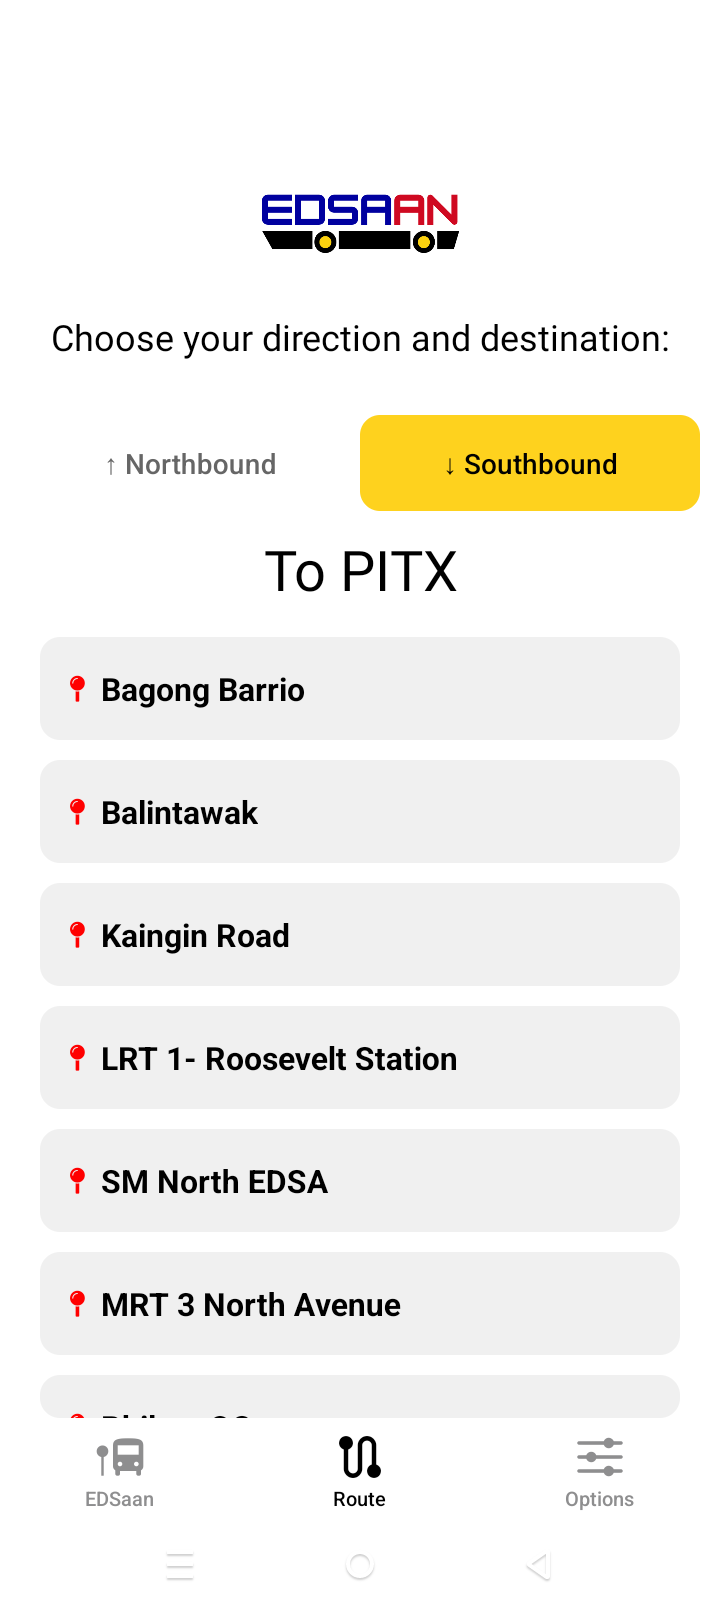
\includegraphics[width=0.25\textwidth]{ICS-template/screenshots/EDSAan_browse.png}
  \caption{Choose Destination Screen}
  \label{fig:yourlabel}
\end{figure}

The user can choose between the Northbound and Southbound directions and then select their destination (Figure 1).

\subsubsection{\textbf{Station Information}}

\begin{figure}[htbp]
  \centering
  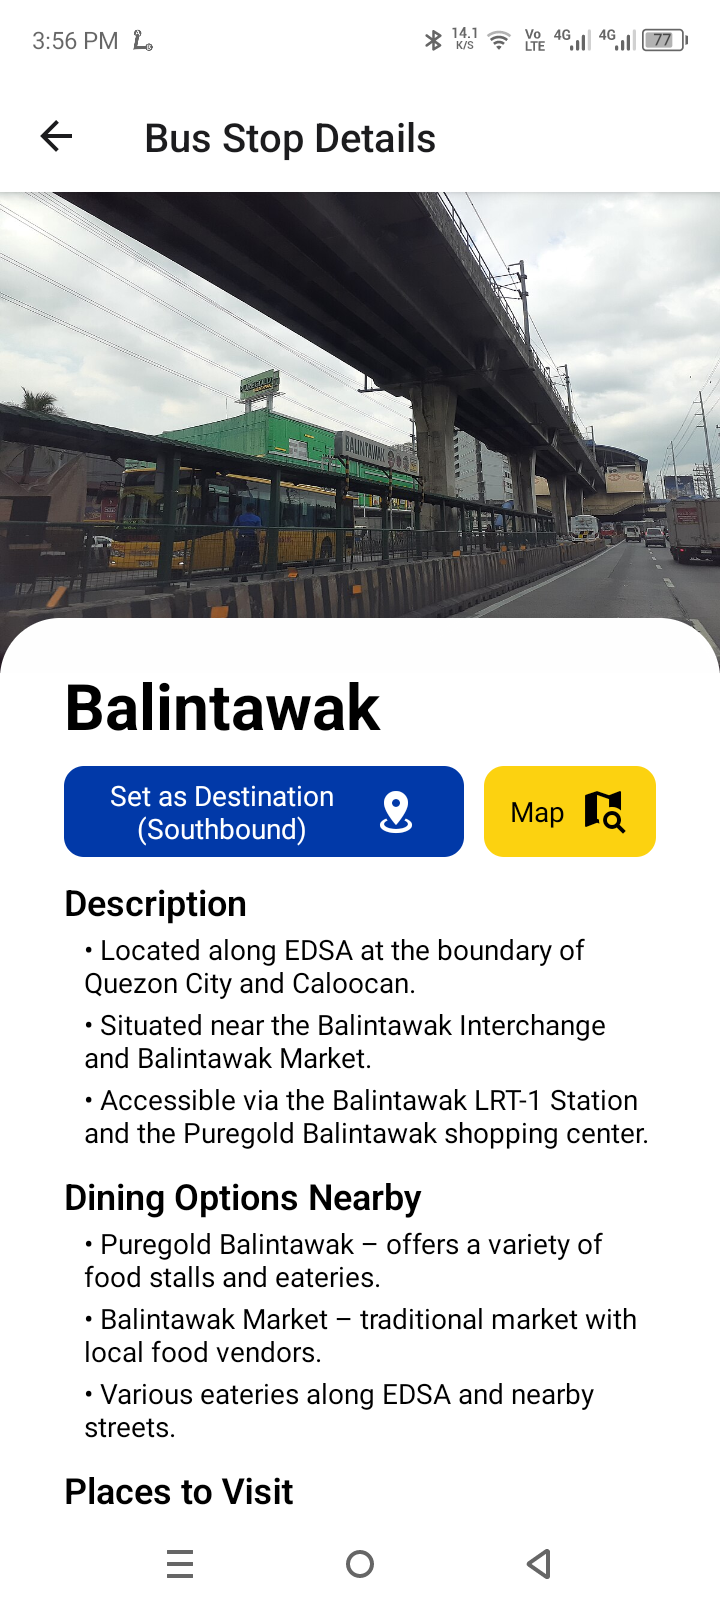
\includegraphics[width=0.25\textwidth]{ICS-template/screenshots/EDSAan_stationinfo.png}
  \caption{Station Information Screen}
  \label{fig:yourlabel}
\end{figure}

Upon pressing a selected station, the user can view its corresponding nearby places to visit, accommodations, and dining places (See Figure 2). There is also a button that views the station inside your default external maps application (Google Maps by default on Android).

\subsubsection{\textbf{Travel Information}}

\begin{figure}[htbp]
  \centering
  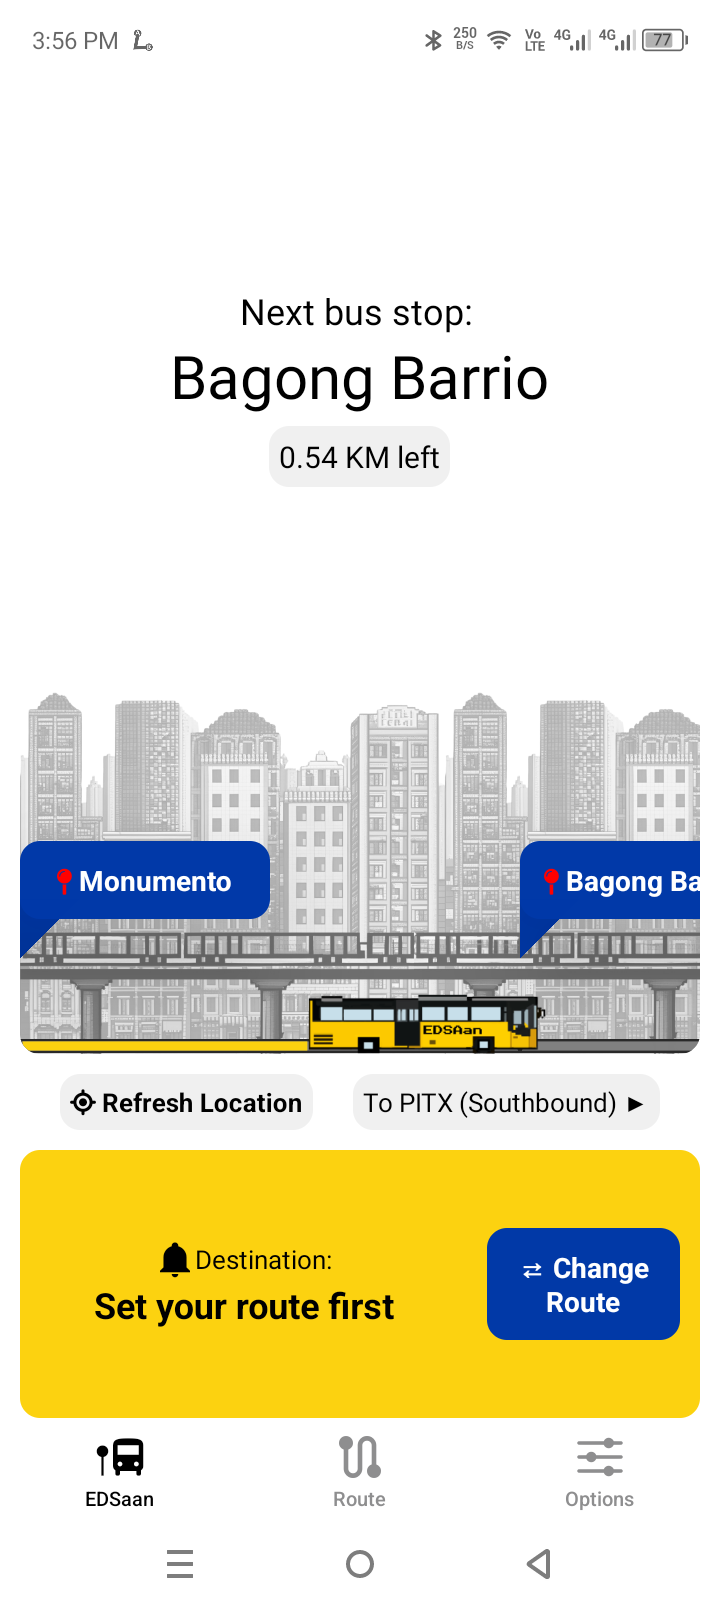
\includegraphics[width=0.25\textwidth]{ICS-template/screenshots/EDSAan_trip.png}
  \caption{Bus Trip Screen}
  \label{fig:yourlabel}
\end{figure}

\begin{figure}[htbp]
  \centering
  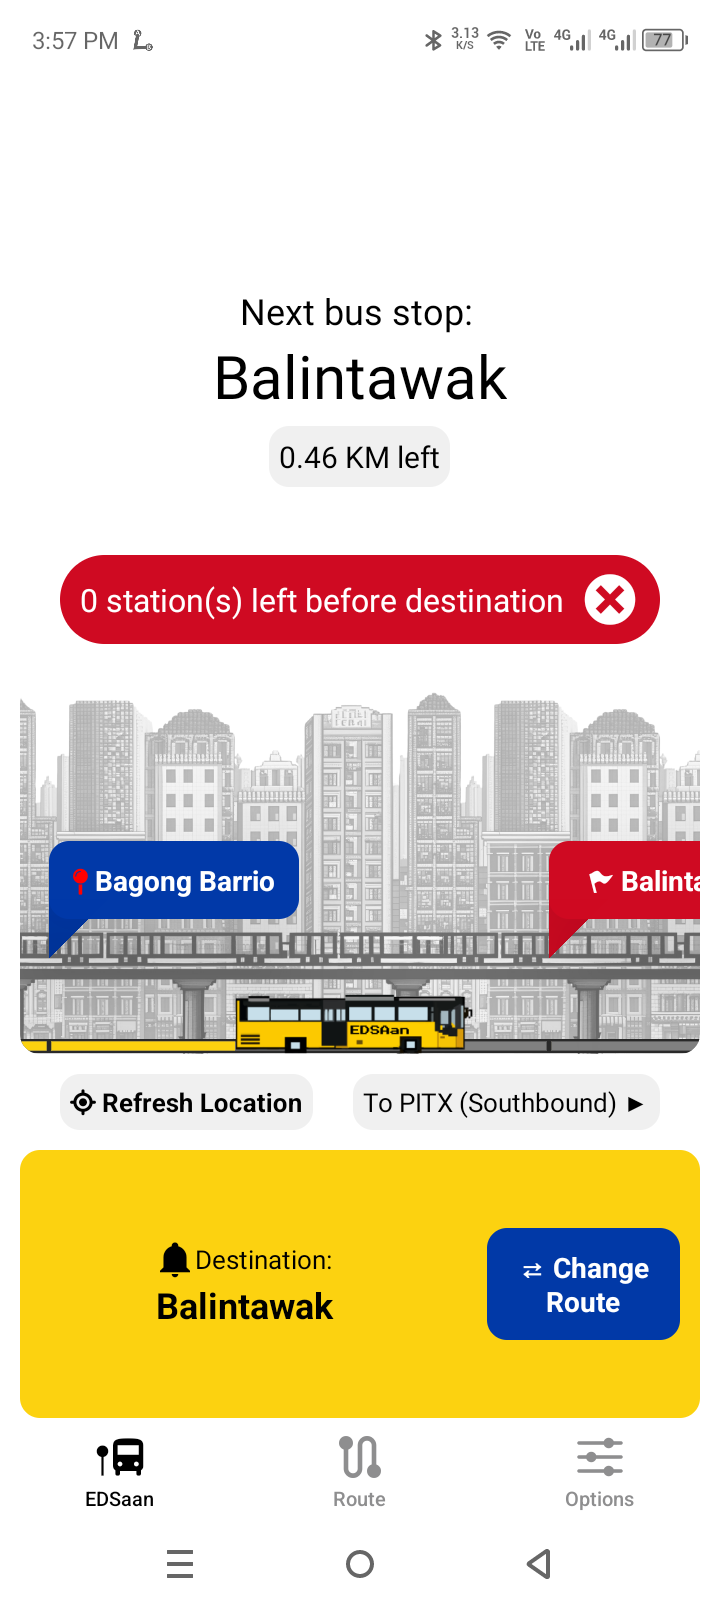
\includegraphics[width=0.25\textwidth]{ICS-template/screenshots/EDSAan_alertbefore.png}
  \caption{Destination Alert Message}
  \label{fig:yourlabel}
\end{figure}

\begin{figure}[htbp]
  \centering
  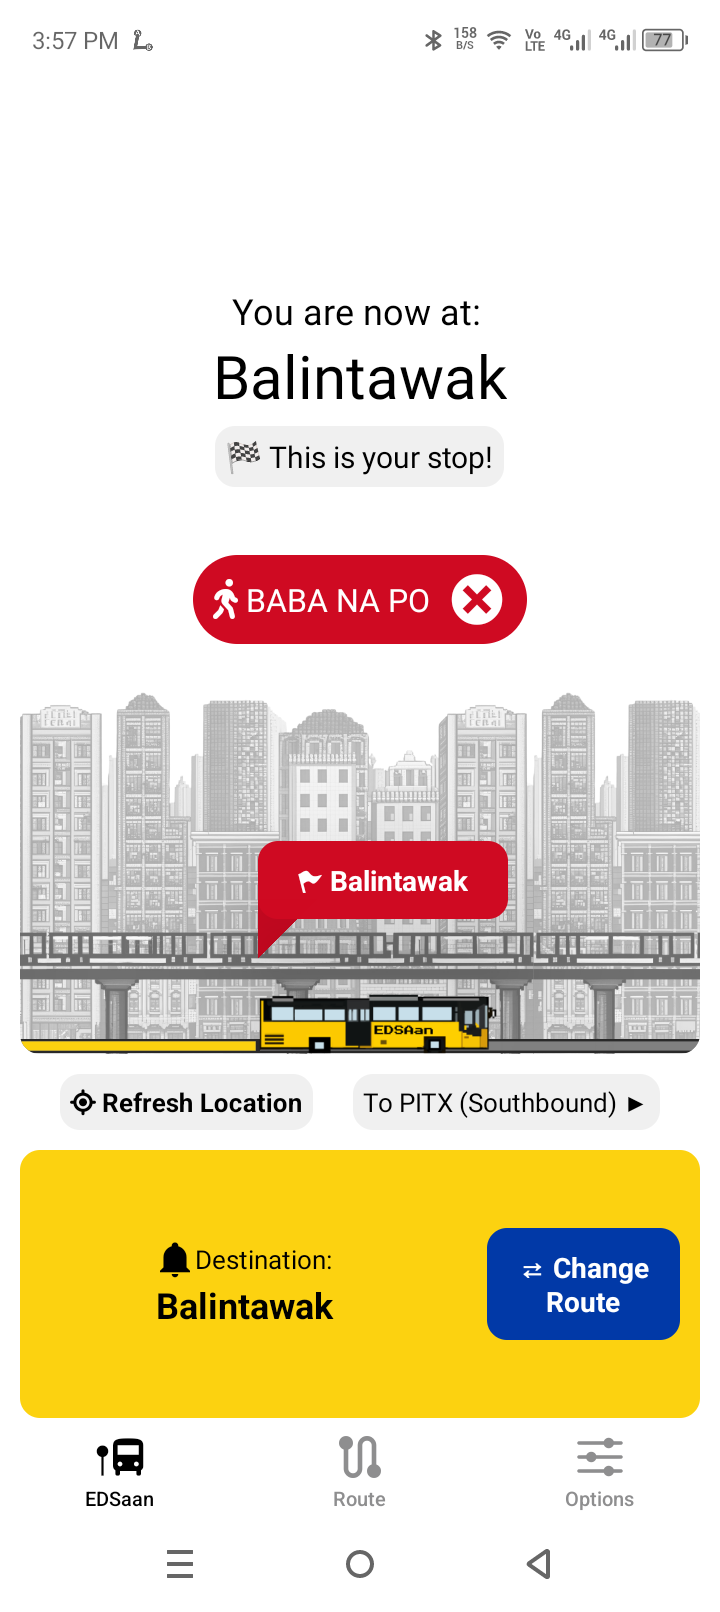
\includegraphics[width=0.25\textwidth]{ICS-template/screenshots/EDSAan_baba.png}
  \caption{Alighting prompt upon reaching destination}
  \label{fig:yourlabel}
\end{figure}

\begin{figure}[htbp]
  \centering
  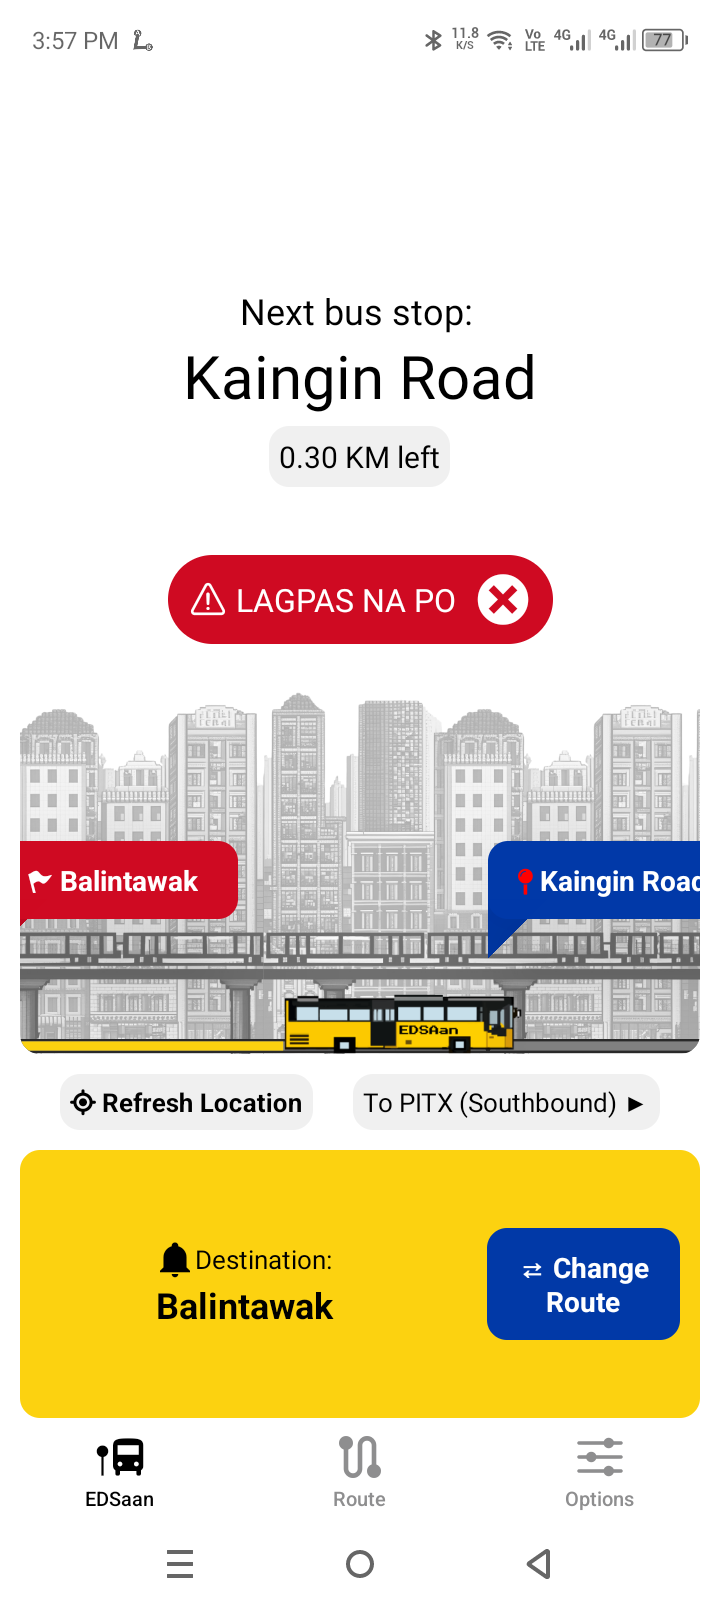
\includegraphics[width=0.25\textwidth]{ICS-template/screenshots/EDSAan_lagpas.png}
  \caption{"LAGPAS" Prompt when you are past your destination}
  \label{fig:yourlabel}
\end{figure}

\begin{figure}[htbp]
  \centering
  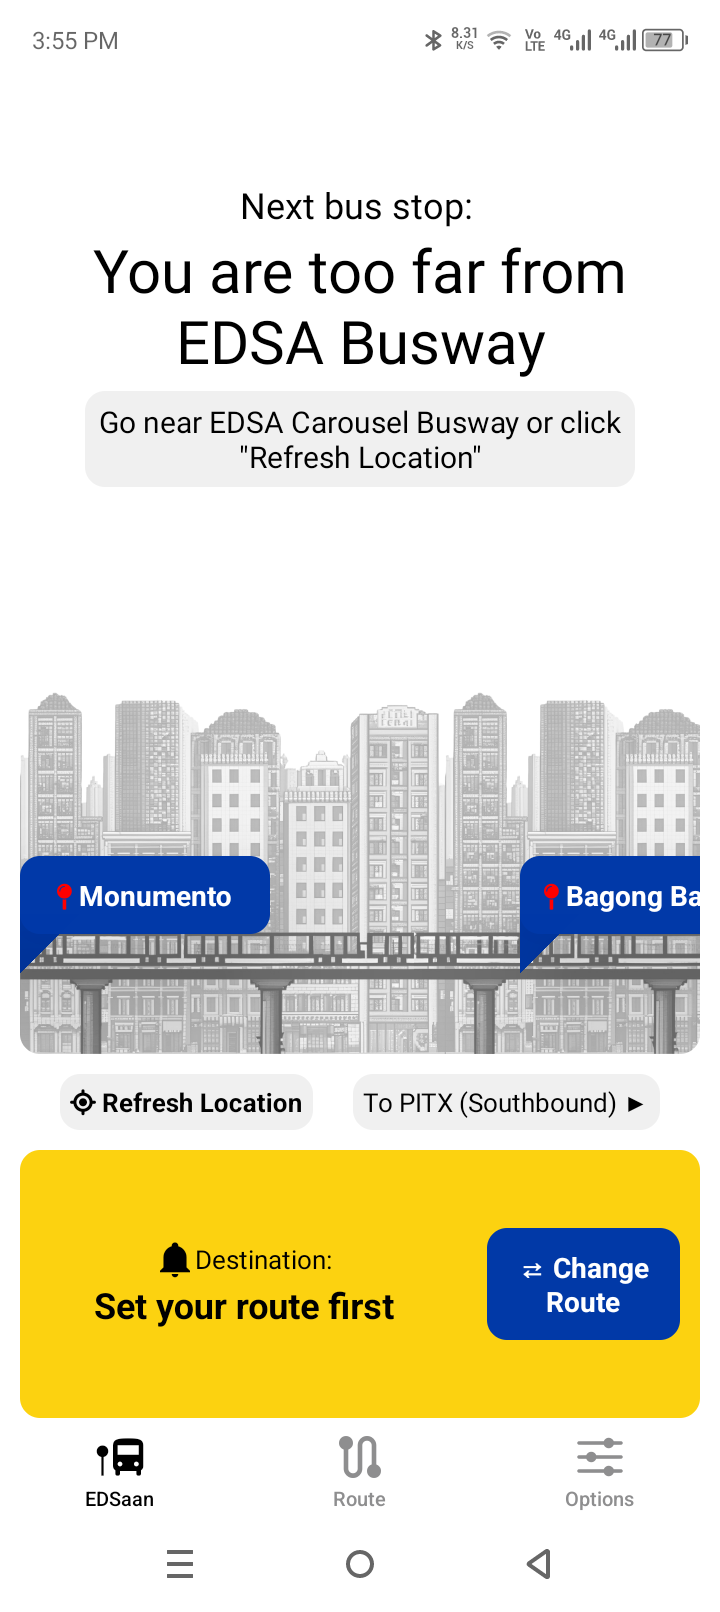
\includegraphics[width=0.25\textwidth]{ICS-template/screenshots/EDSAan_toofar.png}
  \caption{Too far from EDSA}
  \label{fig:yourlabel}
\end{figure}

The bus icon will move along a path that shows your location along the EDSA bus route (See Figure 3). The view is horizontally scrollable, and the stations along the route are also clickable. The station will turn red if it is set as a destination (see Figure 4). The next station will be shown while you travel, along with the remaining distance. The status text will display "BABA NA PO" when you reach your destination (Figure 5) and "LAGPAS NA PO" when you are already past your destination (Figure 6). If you are too far from EDSA, the bus icon will be hidden (Figure 7).

\subsubsection{\textbf{Settings Page}}

\begin{figure}[htbp]
  \centering
  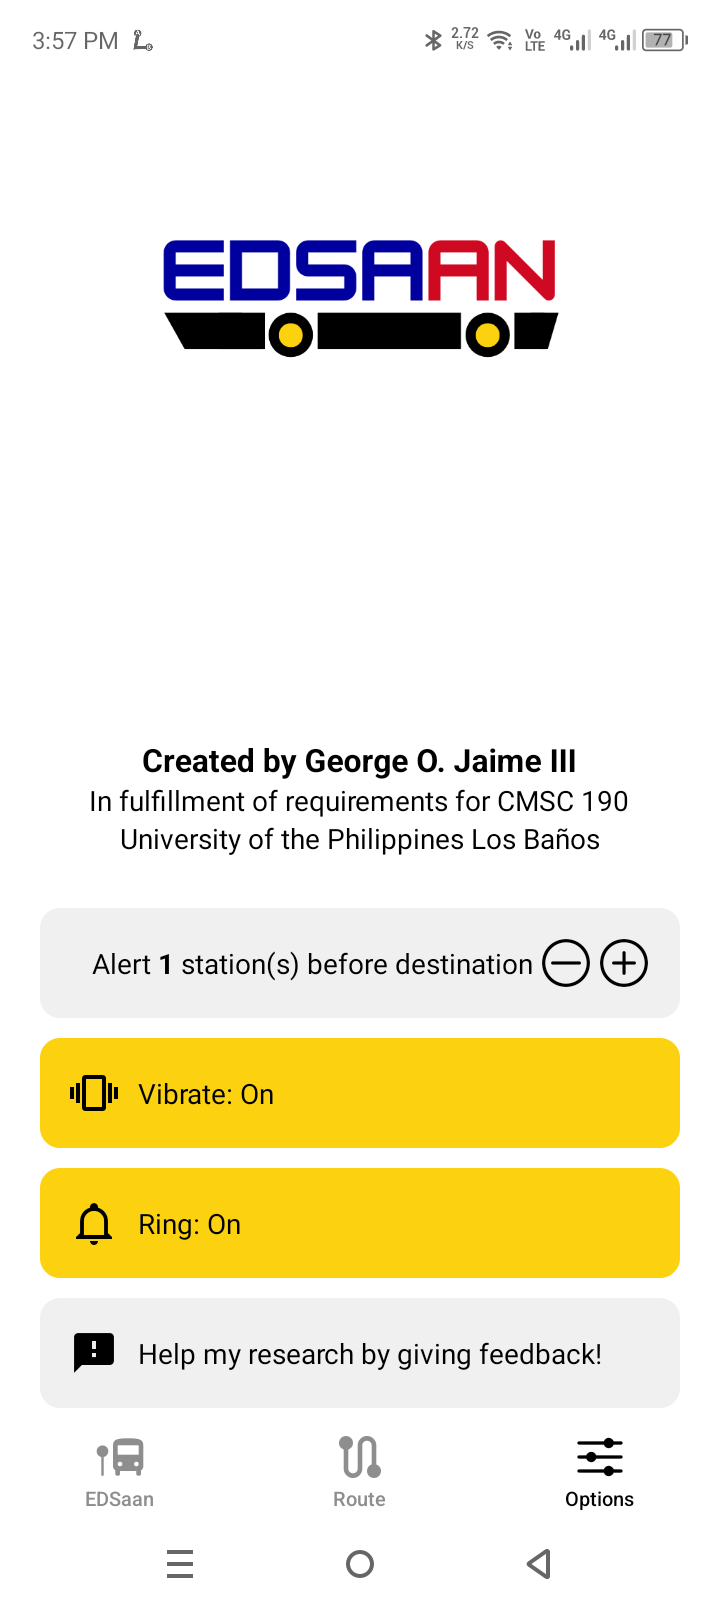
\includegraphics[width=0.25\textwidth]{ICS-template/screenshots/EDSAan_settings.png}
  \caption{Settings Page}
  \label{fig:yourlabel}
\end{figure}

The settings page offer various options (Figure 8). Alerting x stations(s) before the destination will trigger the alerts when you are x stations away from your destination, and the value can be set from 0 to 3. There is also an option to toggle the Vibrate and Ring options on and off separately. This will cause the device to vibrate and/or alarm upon reaching x stations away from destination.

\subsection{User Tests}
The study employed participants that ride the EDSA Busway. Due to the fast paced nature of public transportation, the mobile app installer was distributed online by the means of APK file.

In determining the usability of an offline navigation system in the context of EDSA Carousel, the participants accomplished a Google Form containing the questionnaire after testing EDSAan.

The first part is a 5-point likert-scale questions that addresses the 3 objectives of this study. The questions are as follows:

\begin{enumerate}

\item \textbf{Mobile App Interface Tailored for EDSA Carousel Travel}
    \begin{enumerate}
        \item The app is easy to navigate.
        \item The layout and design help me understand my current location.
        \item The next station and remaining distance are clearly displayed.
        \item I can easily choose a bus stop as my destination.
        \item The sound and vibration notifications are helpful.
    \end{enumerate}

\item \textbf{Effectivity of Smartphone’s Offline GPS}
    \begin{enumerate}
        \item The app functions properly even when offline.
        \item The location shown by the app remains accurate without internet connection.
        \item I can still navigate to my bus stop even when the app is offline.
    \end{enumerate}
\item \textbf{Overall Usability of EDSAan}
    \begin{enumerate}
        \item EDSAan is useful for my daily commute.
        \item I trust EDSAan to notify me at the right bus stop.
        \item The bus station descriptions and nearby places are helpful.
        \item Overall, I am satisfied with the EDSAan app.
    \end{enumerate}

\end{enumerate}

The second part of the questionnaire complied to the Standard Usability Scale, a well known set of questions utilized in evaluating user experience of systems since the 1980s \cite{Ref:010}.

The SUS measures responses using a 5-point likert scale, which enables for five possible responses: strongly disagree, disagree, neutral, agree, strongly agree. It employs the following questions:
\begin{enumerate}
    \item I think that I would like to use this system frequently.
    \item I found the system unnecessarily complex.
    \item I thought the system was easy to use.
    \item I think that I would need the support of a technical person to be able to use this system.
    \item I found the various functions in this system were well integrated.
    \item I thought there was too much inconsistency in this system.
    \item I would imagine that most people would learn to use this system very quickly.
    \item I found the system very cumbersome to use.
    \item I felt very confident using the system.
    \item I needed to learn a lot of things before I could get going with this system.

\end{enumerate}
The scores were normalized as per the specifications of SUS. The scores of the odd-numbered questions were subtracted by 1, and the scores of the even-numbered questions were subtracted from 5. The resulting scores from all items were added together, and then multiplied by 2.5. A score above 68 will be considered above average \cite{Ref:019}.

\subsection{Personal GPS Test and Documentation}
The mobile app was also tested by the researcher on all stations of the EDSA Carousel, with each station recorded on video alongside the mobile app.


\section{Results and Discussion}

This chapter presents the findings from the evaluation of the EDSAan mobile application, as gathered from both user surveys and personal field testing. A combination of quantitative data from Likert-scale questionnaires and the System Usability Scale (SUS), along with qualitative insights from on-site GPS validation, were analyzed to determine the effectiveness, usability, and reliability of the app in the context of commuting via the EDSA Carousel.

\subsection{Survey Response Overview}

A total of 210 participants responded to the evaluation questionnaire for the EDSAan app. These participants were asked to rate several statements across three main objectives using a 5-point Likert scale, where:

1 — Strongly Disagree

2 — Disagree

3 — Neutral

4 — Agree

5 — Strongly Agree

In addition to the objective-specific questions, users also completed the System Usability Scale (SUS), a standardized instrument for evaluating perceived usability.

Out of the 210 responses, 31 were excluded from the analysis due to patterned answering (e.g., marking 'Strongly Agree' on all items, including negatively phrased ones), which contradicted the logic of the scale. This exclusion was conducted to preserve the accuracy and reliability of the score interpretation.

Based on a total estimated population size of 389,579 EDSA Carousel commuters, this sample size yields a margin of error of approximately ±7.32\% at a 95\% confidence level \cite{Ref:020}. This means that if the same survey were repeated multiple times under the same conditions, 95\% of the time, the results would fall within ±7.32\% of the values observed in this study. This level of precision ensures that the results of the evaluation were representative of the general commuting population of the EDSA busway.

\subsection{Objective 1: Mobile App Interface Tailored for EDSA Carousel Travel}
This section assessed how effectively the EDSAan interface supports commuter interactions and navigation through the EDSA Carousel system. The mean scores for each item were as follows:


\begin{center}
\begin{tabular}{ | m{18em} | m{1cm} | } 
  \hline
  The app is easy to navigate.& 4.67 \\ 
  \hline
  The layout and design help me understand my current location. & 4.72 \\ 
  \hline
  The next station and remaining distance are clearly displayed. & 4.69\\ 
  \hline
  I can easily choose a bus stop as my destination. & 4.72\\ 
  \hline
  The sound and vibration notifications are helpful. & 4.65\\ 
  \hline
\end{tabular}
\end{center}

All items received average scores above 4.6, suggesting that users strongly agreed with the usability and clarity of the app’s interface. These results indicate that the app successfully communicates essential travel details and maintains a clear, user-friendly layout. The high score for destination selection and map orientation further confirms the design’s effectiveness in helping commuters plan and track their journey.

\subsection{Objective 2: Effectivity of Smartphone’s Offline GPS}
This section evaluated how well the EDSAan app performs without internet access, particularly in detecting location and guiding users to their stops.

\begin{center}
\begin{tabular}{ | m{18em} | m{1cm} | } 
  \hline
  The app functions properly even when offline. & 4.48 \\ 
  \hline
  The location shown by the app remains accurate without internet. & 4.45 \\ 
  \hline
  I can still navigate to my bus stop even when the app is offline. & 4.50\\ 
  \hline

\end{tabular}
\end{center}

The mean scores indicate that users agreed with the app’s offline functionality, averaging between 4.45 and 4.50. Although slightly lower than interface scores, they still reflect a high level of user confidence in the app’s GPS tracking without requiring a stable data connection, an essential feature for commuters who rely on mobile navigation in transit environments.

\subsection{Objective 3: Overall Usability of EDSAan}
This section focused on the app’s perceived usefulness and overall impact on the commuting experience.

\begin{center}
\begin{tabular}{ | m{18em} | m{1cm} | } 
  \hline
  EDSAan is useful for my daily commute.	 & 4.66 \\ 
  \hline
  I trust EDSAan to notify me at the right bus stop.	 & 4.73 \\ 
  \hline
  The bus station descriptions and nearby places are helpful.	 & 4.76\\ 
  \hline
  Overall, I am satisfied with the EDSAan app.	 & 4.72\\ 
  \hline

\end{tabular}
\end{center}

With all scores above 4.6, users expressed strong satisfaction with the app's overall utility. The highest score (4.76) was given to the helpfulness of bus stop descriptions and nearby landmarks, suggesting that EDSAan contributes meaningfully to trip planning and wayfinding, beyond simple location tracking.

\subsection{System Usability Scale (SUS) Evaluation}
Following the Likert-based evaluations, participants were asked to complete the System Usability Scale (SUS) to assess the app’s overall usability in a standardized format.

After excluding 31 patterned responses, the SUS was computed from the remaining 179 valid entries. The resulting average SUS score was \textbf{85.52}.

According to industry benchmarks, a SUS score above 80.3 is considered “Excellent”, and typically falls within the top 10\% of usability scores for tested applications \cite{Ref:019}. A score of 85.52 places EDSAan in the "Excellent to Best Imaginable" usability range, affirming the app’s strong performance in terms of user experience, ease of use, and satisfaction.

This quantitative finding aligns closely with the Likert-scale responses under Objectives 1 and 3, reinforcing the app's intuitive design and trustworthiness as a commuting companion.

\subsection{Personal GPS Testing and Station Verification}

To further validate the real-world performance of EDSAan, the researcher conducted a comprehensive field test, personally traveling through all 24 EDSA Carousel stations using the app. Each station test was recorded on video, capturing:

\begin{itemize}
    \item Live station recognition by the app
    \item Map synchronization and GPS stability
    \item Offline functionality during route segments
\end{itemize}

The results of this on-site testing confirmed that:
\begin{itemize}
\item The app successfully detected all 24 stations, with accurate naming and location markers.

\item GPS tracking remained functional and accurate, even during periods of poor or absent internet connectivity.

\item No crashes or significant UI lags were observed throughout the full trip.
\end{itemize}

This hands-on verification supports user-reported findings, particularly the high agreement scores in Objectives 1 and 2, by proving that the app functions as intended in actual commuting conditions.

These recordings are available as supporting materials and may be accessed upon request for verification, evaluation, or further review by project stakeholders or academic evaluators.

\subsection{User Feedback and Suggestion}
After the usability evaluation phase, users were invited to share their thoughts and suggestions regarding the EDSAan mobile application. The responses were generally positive, with many praising the app for its usefulness, simplicity, and clear design. Several respondents mentioned that the application was easy to use, with one stating they had mastered its features within a few minutes of use. Another remarked that the interface was “cute and beginner-friendly,” noting that it was “very straightforward.” Many users agreed that EDSAan would be helpful to commuters, especially those who often miss their bus stops or are unfamiliar with the EDSA Carousel route.

One reviewer, who also works as a content moderator for the Google Play Store, mentioned that the application is compliant with Google’s app policies and could be uploaded once ready. They also suggested adding a fare matrix to inform users of estimated costs per trip, while recommending the inclusion of a disclaimer since fare amounts may vary by bus operator. Another user suggested the addition of visible landmarks on the route, as this would help passengers better anticipate their drop-off points. A number of comments expressed excitement about the app’s practical value, urging its official release, noting that it could greatly assist daily commuters.

A particularly valuable insight came from a conductor currently working in the EDSA Carousel Busway. They recommended the addition of more specific stops between major stations such as Mall of Asia (MOA) and PITX—naming W Mall, DFA, Parqal, COD, Ayala Malls, Landmark, and Coastal Mall as commonly used yet unofficial stops that passengers often miss due to lack of information.

A recurring request among respondents was for an iOS version of the application. Many users who own iPhones expressed interest in using EDSAan and hoped for a future release on the App Store.

These responses, along with the quantitative results of the SUS evaluation, provide important direction for further development and refinement of the EDSAan app.

\section{Conclusion and Future Work}
\subsection{Conclusion}
This study focused on creating and testing EDSAan, a mobile application designed to help commuters using the EDSA Carousel bus system in Metro Manila. The app was built to show users their current location, allow them to choose a destination bus stop, and notify them when they are near it, even without an internet connection.

The app was evaluated using two tools: a custom questionnaire based on the app’s goals and the System Usability Scale (SUS). A total of 179 valid responses were used in the analysis, after removing 31 patterned or inconsistent answers to maintain the accuracy of the results. Based on the data, users rated the app very positively. The interface-related questions had high average scores, showing that users found the app easy to use and understand. The offline GPS feature also received favorable scores, which means the app worked well even without internet access. The overall usability was rated highly too, especially in terms of satisfaction and usefulness. The SUS score was 85.52, which is considered excellent and shows that the app meets high standards in usability.

In addition to the survey, the researcher tested the app personally across all 24 EDSA Carousel stations. The trips were recorded to show how the app performs in real conditions. These tests confirmed that the app gave accurate location updates and helpful alerts throughout the route.

Overall, EDSAan was able to meet its goals. It is a helpful tool for commuters and provides a smooth and reliable experience for those using the EDSA Carousel.

\subsection{Future Work}
Although the app has successfully met its current objectives, there are still ways it can be improved or expanded in the future.

One suggestion from a user, who is a conductor of the EDSA Carousel, is to include more bus stops between key locations such as MOA to PITX. Stops like Wmall, DFA, Parqal, Cod, Ayala Malls Landmark, Coastal, and PITX could help passengers who are unaware of the opportunity to disembark at specific places along the route. This could prevent passengers from missing their stops and enhance the app's usefulness for commuters.

Another frequent request from users is the development of an iOS version of the app. Since many commuters use Apple devices, an iOS version would significantly expand the app’s reach and ensure that more people benefit from its features.

Additionally, it would be helpful to add real-time bus tracking in partnership with agencies like the Department of Transportation (DOTr) or the Land Transportation Franchising and Regulatory Board (LTFRB). This would make the app even more accurate.

In the future, the app could also help transport planners. With user permission, the data gathered could give insights to improve bus routes and public services. It also has the potential to serve as another application for train lines in the Philippines.

By working on these improvements, EDSAan can grow into a more complete and useful app for all types of commuters in the country.

% BIBLIOGRAPHY
\bibliographystyle{IEEE/IEEEtran}
\bibliography{cs190-ieee}


% ACKNOWLEDGMENT
\section*{Acknowledgment}
I would like to express my deepest gratitude to Prof. Concepcion L. Khan, my Special Problem adviser, for her valuable insights and for guiding the direction of this project. Her support and feedback were instrumental in shaping this study. \hfill \\

I am also sincerely thankful to my loving girlfriend, Armiel Grace F. Rivera, for her help documenting the mobile application at all 24 EDSA Carousel stations. Her support and dedication played a vital role in completing this work. \hfill \\

I would also like to express my gratitude to my cousin, Gerlyn Ramos Madrid, for providing me with the laptop I used to develop and complete this research project. Her support enabled me to carry out the technical work required for this study. \hfill \\\

To my friend Armi Angelika Dulay, thank you for the financial help you extended during difficult times. Your generosity made it possible for me to continue and complete this research. \hfill \\

To Faye Fernando, I am grateful for the opportunity you gave me to work while studying. Your support helped me manage my academic and professional responsibilities. \hfill \\

Lastly, I would like to thank my family for their unwavering support, understanding, and encouragement throughout this journey. Their presence has always been my foundation.

\begin{biography}[{
\includegraphics{./yourPicture.eps}}]{George O. Jaime III}
is a Bachelor of Science in Computer Science student at the University of the Philippines Los Baños. Originally from San Jose del Monte, Bulacan, he is a working student employed as a bartender in Makati City, balancing his academic and professional responsibilities with dedication and resilience.
\end{biography}

\end{document}
 
